% ==============================================================================================================
\section{Quantum Coupled Cluster}\label{sez:quantum-coupled-cluster}
% FIXME
Riuscire a costruire un ansatz che approssimi lo stato fondamentale è determinante per il successo di algoritmi variazionali quantistici come VQE, allo stesso tempo rimane l'importanza chiave di costruire la funzione d'onda in modo efficiente.

Il metodo \inglese{quantum Unitary Coupled Cluster} ($q$-UCC), ispirato alla sua controparte classica UCC (sez. \ref{subsec:coupled-cluster}), offre una soluzione scalabile, oltre che fisicamente motivata. 
Inoltre, a differenza dei metodi CC classici, l'energia su uno stato $q$-UCC può essere determinata variazionalmente \cite{Anand_2022}.

% ..............................................................................................................
\subsubsection{Eccitazioni troncate}

In maniera del tutto analoga alla variante classica CC (eq. \ref{eqn:CC-variants}), $q$-UCC permette il troncamento sistematico delle eccitazioni. In questo studio si prenderanno in esame le varianti $q$-UCCS, $q$-UCCD e $q$-UCCSD

\begin{subequations}\label{eqn:q-UCC-variants}
\begin{align}
    \ket{\Phi_{q-\text{CCS}}}  &= e^{\hat{T}_1-\hat{T}_{1}^{\dagger}} \ket{\Phi_{\text{HF}}}
    \\
    \ket{\Phi_{q-\text{CCD}}}  &= e^{\hat{T}_2-\hat{T}_{2}^{\dagger}} \ket{\Phi_{\text{HF}}}
    \\
    \ket{\Phi_{q-\text{CCSD}}} &= e^{\hat{T}_1-\hat{T}_{1}^{\dagger} + \hat{T}_2-\hat{T}_{2}^{\dagger}} \ket{\Phi_{\text{HF}}}
\end{align}
\end{subequations}



% --------------------------------------------------------------------------------------------------------------
\subsection{Implementazione}

Il primo passo nell'implementazione dell'ansatz q-UCC è la costruzione dell'operatore unitario $\mathsf{U}$, presentato già nell'equazione~\ref{eqn:unitary-coupled-cluster}:

\begin{equation}\label{eqn:unitary-UCC-transformation}
    \mathsf{U} \equiv e^{\hat{T} - \hat{T}^{\dagger}} = 
    e^{\sum_{k} \hat{T}_k - \hat{T}^{\dagger}_{k}}
\end{equation}

dove $\hat{T}$ è l'operatore di cluster (eq. \ref{eqn:cluster-operator}). Quindi, $\mathsf{U}$ deve essere tradotto in operazioni eseguibili su un dispositivo quantistico.

% ..............................................................................................................
\subsubsection{Approssimazione di Trotter}

I vari ordini di eccitazioni $\hat{T}_k$ non commutano tra loro, perciò è necessario ricorrere a delle approssimazioni; in questo caso, si ricorre alla formula di Trotter $e^{\hat{A}+\hat{B}} \approx e^{\hat{A}}e^{\hat{B}}$:

\begin{equation}\label{eqn:UCC-Trotter}
    \mathsf{U} \approx 
    \prod_k e^{\hat{T}_k - \hat{T}^{\dagger}_{k}} = \prod_k U_k
\end{equation}


% O PIÙ SPECIFICO?
\begin{equation}\label{eqn:formula-di-Trotter}
    e^{\hat{A}+\hat{B}} \approx \lim_{t\rightarrow\infty} 
    \left( 
        e^\frac{A}{t} e^\frac{B}{t}
    \right)^t
\end{equation}

applicato a $\mathsf{U}$

\begin{equation}\label{eqn:UCC-Trotter-2}
    \mathsf{U} \approx 
    \left(
        \prod_i e^{\frac{1}{t} \hat{T}_i - \hat{T}^{\dagger}_{i}} 
    \right)^t
\end{equation}

ciò permette di scomporre $\mathsf{U}$ in una produttoria di operatori unitari $U_k$, che poi possono essere espressi in termini di quantum gates in modo efficiente, anche se, in generale, questo processo porta a circuiti piuttosto grandi.

Ad esempio, nel caso $q$-UCCSD si ha:

\begin{equation}\label{eqn:UCCSD}
    \mathsf{U}_{SD} = 
    e^{\hat{T}_1 - \hat{T}^{\dagger}_{1} + \hat{T}_2 - \hat{T}^{\dagger}_{2}}
\end{equation}

applicando l'approssimazione di Trotter ed esplicitando gli operatori di eccitazione con le relazioni~\ref{eqn:cluster-operator}:

\begin{equation}
\begin{aligned}
    \mathsf{U}_{SD}
    &= e^{\hat{T}_1 - \hat{T}^{\dagger}_{1}} e^{\hat{T}_2 - \hat{T}^{\dagger}_{2}}\\
    &= 
    \exp\left(
        {\sum_{a,r} \theta_{a}^{r}\,( a^{\dagger}_r a_a - a^{\dagger}_a a_r )}
        \right)
    \exp\left(
        \sum_{\substack{a<b\\r<s}} \theta_{ab}^{rs}\, 
        (a^{\dagger}_r a^{\dagger}_{s} a_a a_b - a^{\dagger}_b a^{\dagger}_{a} a_s a_r)
        \right)
\end{aligned}
\end{equation}

che si può scomporre con Trotter ulteriormente:

\begin{equation}
    \mathsf{U}_{SD} = 
    \prod_{a,r} \exp\left({\theta_{a}^{r}\,( a^{\dagger}_r a_a - a^{\dagger}_a a_r )}\right)
    \prod_{\substack{a<b\\r<s}} 
    \exp\left({\theta_{ab}^{rs}\,(a^{\dagger}_r a^{\dagger}_{s} a_a a_b - a^{\dagger}_b a^{\dagger}_{a} a_s a_r)}\right)
\end{equation}


A questo punto si può procedere con la mappatura degli operatori fermionici a \inglese{qubit operators}, utilizzando un qubit mapper come le trasformazioni di Jordan-Wigner \cite{Barkoutsos_2018}.

% ..............................................................................................................
\subsubsection{Circuiti}
% FIXME: lo screenshot non ha qualità sufficiente
I circuiti che ne risultano sono:

\begin{figure}[H]
    \centering
    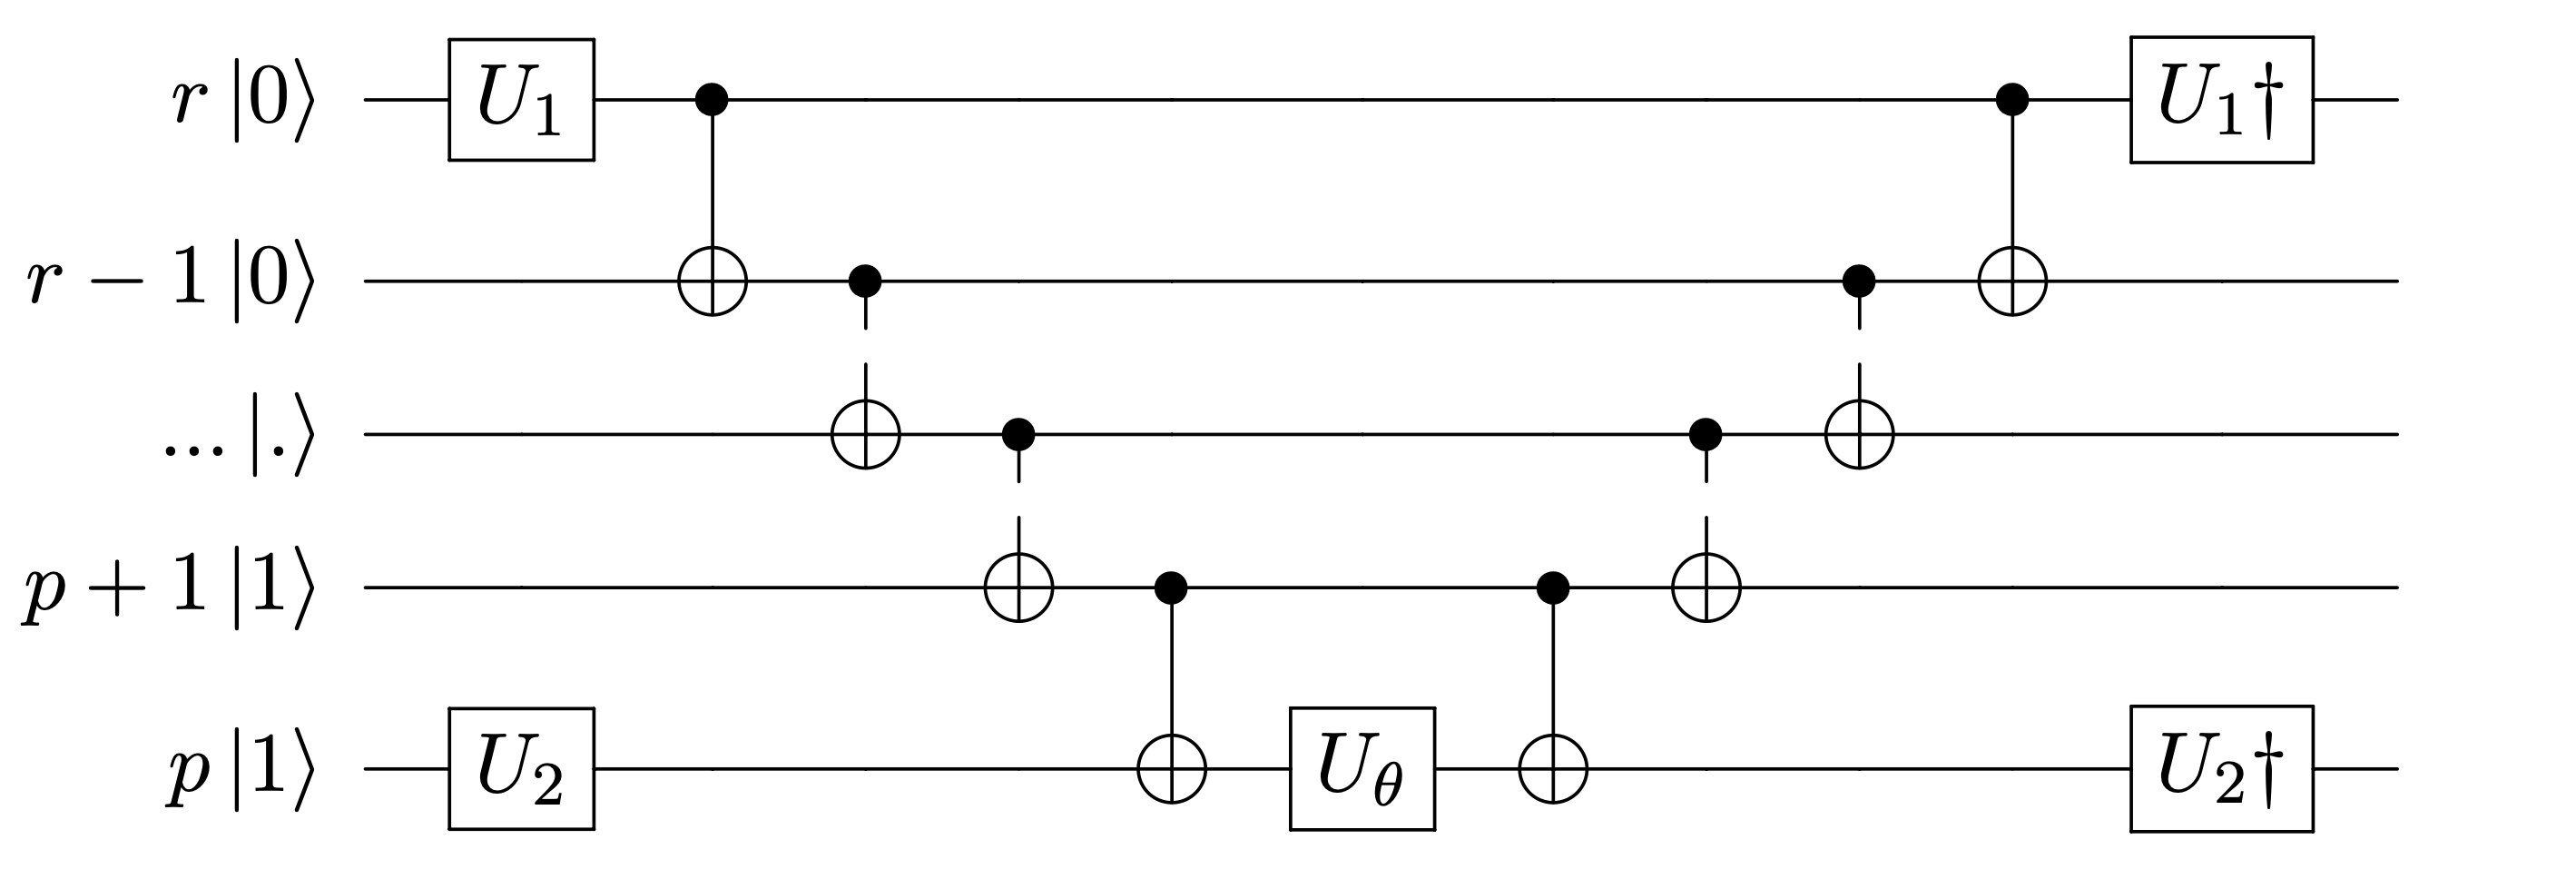
\includegraphics[width=0.8\textwidth]{Immagini/Capitolo_2/ucc_singles.png}
    \caption{Esponenziazione eccitazioni singole \cite{Carobene_2021}.}
    \label{fig:eccitazioni-singole}
\end{figure} 

con $(U_1,U_2)\in\{(Y,H),(H,Y)\}$, per l'esponenziazione di $\hat{T}_1-\hat{T}_{1}^{\dagger}$;

\begin{figure}[H]
    \centering
    \hspace{0.5cm}
    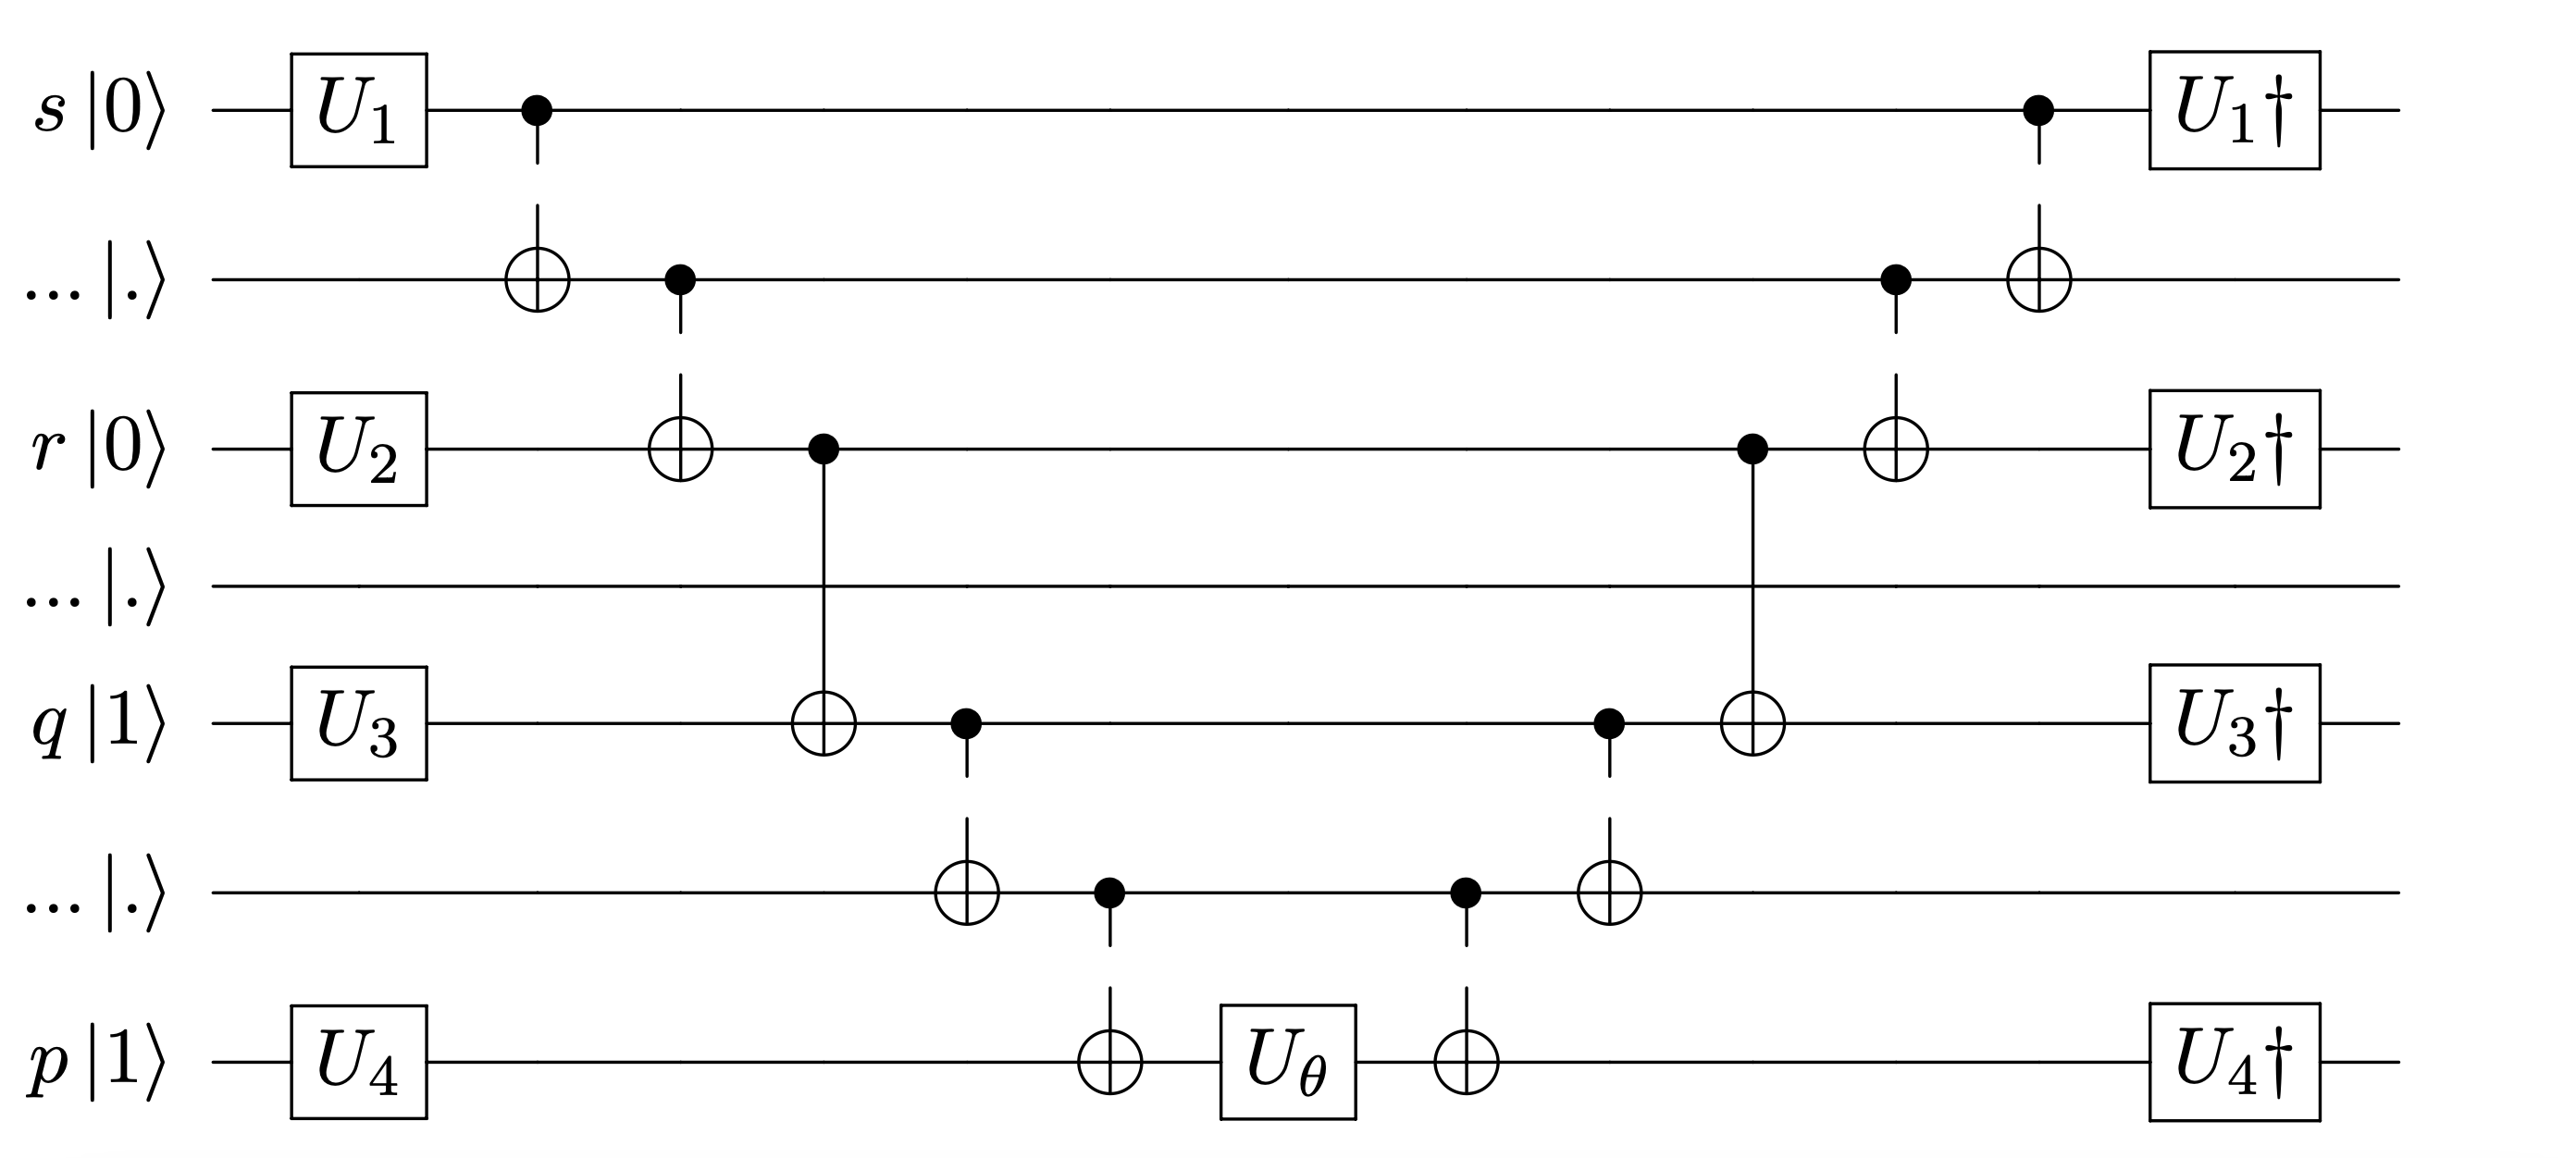
\includegraphics[width=0.8\textwidth]{Immagini/Capitolo_2/ucc_doubles.png}
    \caption{Esponenziazione eccitazioni doppie \cite{Carobene_2021}.}
    \label{fig:eccitazioni-doppie}
\end{figure} 

dove 
\begin{align*}
    (U_1,U_2,U_3,U_4)\in\{&(H,H,Y,H),(Y,H,Y,Y),(H,Y,Y,Y),(H,H,H,Y),\\
    &(Y,H,H,H),(H,Y,H,H),(Y,Y,Y,H),(Y,Y,H,Y)\}
\end{align*}

per l'esponenziazione di $\hat{T}_2-\hat{T}_{2}^{\dagger}$.

Per formare l'ansatz UCCSD basterà concatenare questi due circuiti allo stato HF di partenza.

% --------------------------------------------------------------------------------------------------------------
\subsection{Pair Unitary Coupled Cluster Doubles (pUCCD)}\label{subsec:pUCCD}

Nell'approccio pUCCD si selezionano soltanto le eccitazioni doppie e si impone che queste agiscano sempre su coppie di elettroni. Se si studia un sistema con numero pari di elettroni nello stato fondamentale e se ne considerano i $K$ orbitali spaziali, si può definire l'operatore di eccitazione doppia accoppiata:

\begin{equation}\label{eqn:operatore-paired-cluster}
    \hat{T}_{\text{pCCD}} = \sum_{a,r} 
    \theta_{a_\alpha a_\beta}^{r_\alpha r_\beta}\,
    a^{\dagger}_{a_\alpha} a^{\dagger}_{a_\beta} a_{r_\alpha} a_{r_\beta}
\end{equation}

dove $a,r$ stavolta indicizzano gli orbitali spaziali, all'interno dei quali $\alpha,\beta$ indicano lo spin. La funzione d'onda pUCCD è definita così:

\begin{equation}
    \ket{\text{pUCCD}} = e^{\hat{T}_{\text{pCCD}} - \hat{T}_{\text{pCCD}}^{\dagger}} \ket{HF}
\end{equation}

dove si è usato $\ket{HF}$ per indicare la soluzione di Hartree-Fock di riferimento. Questo appaiamento determina una sostanziale diminuzione nel numero di parametri variazionali e di gate richiesti, al prezzo di una minore capacità di rappresentare il problema in esame. Esiste tuttavia una strategia correttiva: i risultati ottenuti con pUCCD, in particolare quelli relativi all'energia di dissociazione, migliorano significativamente se corretti tramite \inglese{orbital optimization}, con cui si può compensare l'omissione dei termini di eccitazione singola. 

% ..............................................................................................................
\subsubsection{Orbital Optimized pair Unitary Coupled Cluster Doubles (oo-pUCCD)}
% FIXME
L'ottimizzazione orbitale consiste nell'applicare un'operatore di rotazione $\hat{R}=e^{-\hat{\mathcal{K}}}$, che agisce sugli orbitali di spin $\{\phi_k\}$ \cite{Sokolov_2020,Zhao_2023}

\begin{equation}\label{eqn:ansatz-oo-pUCCD}
    \ket{\text{oo-pUCCD}} = e^{-\hat{\mathcal{K}}} \ket{\text{pUCCD}}
\end{equation}

$\hat{\mathcal{K}}$ è un'operatore \textbf{anti-hermitiano} $\hat{\mathcal{K}}^\dagger = - \hat{\mathcal{K}}$, che sostanzialmente rende conto delle eccitazioni singole precedentemente trascurate \cite{Mizukami_2020}. 

\begin{equation}\label{eqn:operatore-K}
    \hat{\mathcal{K}} = \sum_{p<q} \mathcal{K}_{pq} (a_{q}^{\dagger}a_{p} - a_{p}^{\dagger}a_{q})
\end{equation}

Il valore di aspettazione diventa:

\begin{equation}\label{eqn:energia-oo-pUCCD}
    \bra{\text{pUCCD}} e^{\hat{\mathcal{K}}} \hat{H} e^{-\hat{\mathcal{K}}} \ket{\text{pUCCD}} 
\end{equation}

e in seguito alla trasformazione degli orbitali, vengono modificati gli integrali ad uno (eq. \ref{eqn:integrale-un-elettrone}) e due corpi (eq. \ref{eqn:integrale-due-elettroni}) utilizzati per generare l'hamiltoniana di seconda quantizzazione:

\begin{subequations}\label{eqn:trasformazione-integrali}
\begin{align}
    \tilde{h}_{pq}   &= \sum_{uv}\; C_{up}^{\star}\, h_{uv} \,C_{vq}\\
    \tilde{g}_{pqrs} &= \sum_{uvxy} C_{up}^{\star}C_{vq}^{\star}\, g_{uvxy} \,C_{xr}C_{ys}
\end{align}
\end{subequations}

dove si è indicato $C_{pq} = [ e^{\hat{-\mathcal{K}}} ]_{pq}$. Per determinare il set di $\{\mathcal{K}_{pq}\}$ che minimizzano l'energia (eq. \ref{eqn:energia-oo-pUCCD}) si costruisce il circuito oo-pUCCD concatenando a pUCCD l'operatore $e^{\hat{\mathcal{K}}}$, seguendo gli stessi passaggi descritti alla Sezione~\ref{sez:quantum-coupled-cluster}. 
Dunque si procede con la minimizzazione variazionale tramite VQE (sez. \ref{subsec:VQE}) ma stavolta, dopo ciascuna ottimizzazione dei parametri, vengono ricalcolati gli integrali utilizzando le relazioni~\ref{eqn:trasformazione-integrali} e l'hamiltoniana viene trasformata di conseguenza. 

% ==============================================================================================================
\section{Hardware efficient ansatzes}\label{sez:hardware-efficient}

UCC rientra nella categoria degli ansatze \inglese{problem inspired}, costruiti a partire da considerazioni sulla fisica del problema da risolvere. Funzioni d'onda di questo tipo promettono di fornire risultati soddisfacenti, ma possono risultare impossibili da implementare, nelle condizioni attuali, per applicazioni aldilà delle semplici dimostrazioni \cite{Bharti_2022}. 

L'obiettivo primario degli ansatze \inglese{hardware-efficient} (HEA) è minimizzare profondità e numero di operazioni del circuito per rispondere alle limitazioni dei dispositivi NISQ \cite{Leone_2024}. Forme variazionali di questo tipo sacrificano l'attinenza con la teoria fisica sottostante, perciò vengono dette \inglese{problem agnostic}.

% ..............................................................................................................
\subsubsection{Ansatz rotazionali \cite{qiskit_TwoLocal}}

Un esempio di forme variazionali \inglese{hardware-efficient} sono gli \textbf{ansatz rotazionali}, così chiamati perché i loro circuiti sono costituiti da operazioni di rotazione su singolo qubit, alternate ad operazioni di entanglement. 
Un semplice schema per questo ansatz si basa sulle rotazioni parametriche $R_x(\theta)$, $R_y(\theta)$ e $R_z(\theta)$, generate attraverso l'esponenziazione delle matrici $X$, $Y$ e $Z$ introdotte alla Sezione~\ref{subsec:gates}.

\begin{subequations}\label{eqn:rotazioni-parametriche}
\begin{align}
    R_x &\equiv e^{-iX\frac{\theta}{2}} = 
    \begin{pmatrix}
        \cos\frac{\theta}{2}   &-i\sin\frac{\theta}{2}\\
        -i\sin\frac{\theta}{2} &\cos\frac{\theta}{2}
    \end{pmatrix}\\
    R_y &\equiv e^{-iY\frac{\theta}{2}} = 
    \begin{pmatrix}
        \cos\frac{\theta}{2} &-\sin\frac{\theta}{2}\\
        \sin\frac{\theta}{2} &\cos\frac{\theta}{2}
    \end{pmatrix}\\
    R_z &\equiv e^{-iZ\frac{\theta}{2}} = 
    \begin{pmatrix}
        e^{-i\frac{\theta}{2}} &0\\
        0  &e^{i\frac{\theta}{2}}
    \end{pmatrix}
\end{align}
\end{subequations}

poiché queste rotazioni appartengono al gruppo delle matrici speciali unitarie di rango 2 [SU(2)] \cite{McMillan_2019}, rappresentate da matrici 2$\times$2 unitarie con determinante 1, gli ansatze rotazionali di questo tipo vengono soprannominati EfficientSU(2).  

Un esempio di circuito EfficientSU(2) su 3 qubit che impiega soltanto $R_y$ e $R_z$ potrebbe essere:

\begin{figure}[H]
\begin{center}
\begin{quantikz}
\gate{R_y(\theta_1)} & \gate{R_z(\theta_3)} & \ctrl{1} & \ctrl{2} & \qw      & \gate{R_y(\theta_6)} & \gate{R_z(\theta_9)}\\
\gate{R_y(\theta_2)} & \gate{R_z(\theta_4)} & \targ{ } & \qw      & \ctrl{1} & \gate{R_y(\theta_7)} & \gate{R_z(\theta_10)}\\
\gate{R_y(\theta_3)} & \gate{R_z(\theta_5)} & \qw      & \targ{ } & \targ{ } & \gate{R_y(\theta_8)} & \gate{R_z(\theta_11)}
\end{quantikz}
\end{center}
\caption{Esempio di ansatz rotazionale.}
\end{figure}

Per migliorare la convergenza, è possibile aumentare i parametri circuitali ripetendo questo insieme di rotazioni ed entanglement un numero $D$ arbitrario di volte, al prezzo di una maggiore profondità. 

